\chapter{Tools installation}
\label{chap:ch2}

\section{Alpha-Beta-CROWN}
\label{sec:ch2sec1}

\par Alpha Beta Crown serves as a neural network verifier based on an efficient linear bound propagation framework and branch and bound \cite{abc}. Setting it up involved a two-step process: first, installing Miniconda and then the tool itself. There were no complications in the first part, as there is an executable file available on their official site that takes care of the entire setup once run. However, the latter part, involving the tool's installation, presented numerous complications.

\par The setup of Alpha Beta Crown followed their "Installation and Setup" section outlined on GitHub. The first command was supposed to clone their GitHub repository including "auto\_LiRPA", an essential component for the tool's functionality. Despite running this command, only the tool's files were retrieved due to permission denials that restricted access to the second GitHub repository. Resolving this required an additional step: manually obtaining the missing necessary files and placing them in their indicated location. The next phase involved creating the conda environment using the specified command, which led to an error that can be observed in figure \ref{Fig_Err}. 

\begin{figure}[htbp]
	\centering
		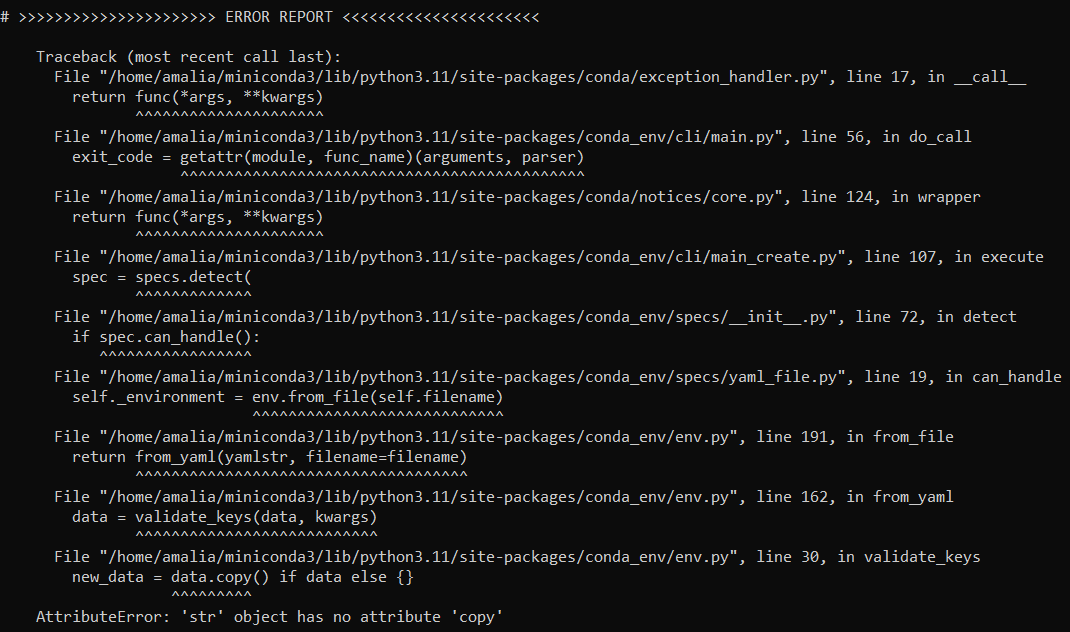
\includegraphics[width=10cm]{./Figures/ToolErr.png}
	\caption{Creating conda environment error}
	\label{Fig_Err}
\end{figure}

\par This error consumed a considerable amount of time, as the error message initially suggested an issue with the script. After extensive investigation, the root cause was traced to the configuration file. Instead of containing the necessary configuration for the conda environment, it referenced another configuration file by name. After resolving the configuration file issue, the installation of the tool seemed successful. However, when attempting to run it, another problem emerged indicating a missing library, "auto\_LiRPA". Although the necessary files existed, the error message revealed a discrepancy in the file path. It seemed that the correct location for this library was wrongly specified. With this adjustment, the setup concluded, and the tool run successfully.
 

\section{Marabou}
\label{sec:ch2sec2}